\chapter{Tổng quan về điện tâm đồ}
\thispagestyle{fancy}

\section{Những khái niêm cơ bản về điện tâm đồ}
\subsection{Định nghĩa}
Điện tâm đồ (ECG) là một đường cong ghi lại các biến thiên của các điện lực do tim phát ra trong khi hoạt động co bóp. Ngoài đo tốc độ và nhịp điệu của tim thì điện tâm đồ còn cung cấp thêm những bằng chứng gián tiếp về lưu lượng máu truyền đến tim. Một xung điện sẽ được tạo ra từ các tế bào trong buồng tim khi tim hoạt động và những tín hiệu khi những xung điện này theo một hệ thống dẫn truyền đi qua tim sẽ được điện tâm đồ ghi lại. Nhờ có điện tâm đồ mà các bác sĩ có thể phát hiện ra được những bệnh lý về tim như loạn nhịp tim, đau thắt ngực,…Thỉnh thoảng, việc tiến hành điện tâm đồ cũng được coi như một xét nghiệm thường quy tại các bệnh viện.
\begin{center}
    \begin{figure}[htp]
    \begin{center}
    %  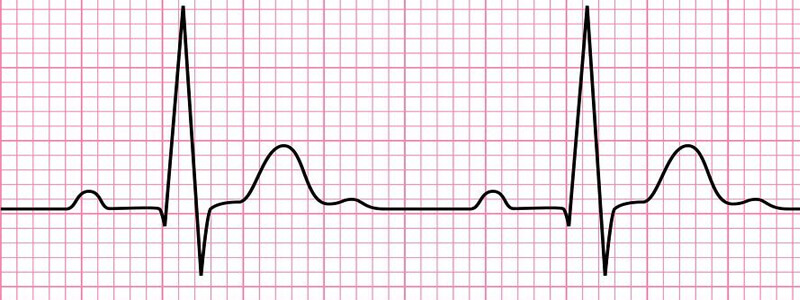
\includegraphics[scale=.]{image/week1/intro.jpg}
     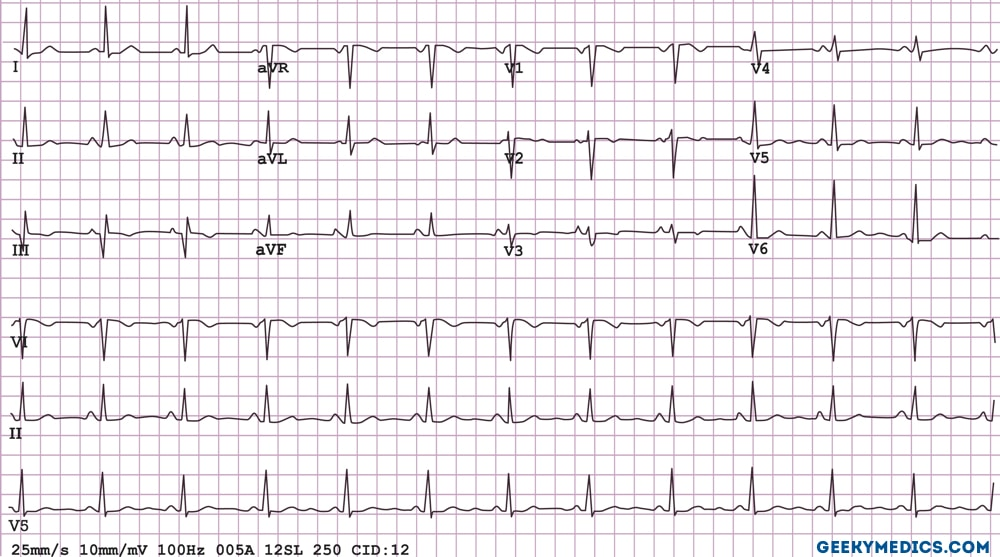
\includegraphics[scale=.35]{image/chapter1/Normal-ECG-SCALED-DOWN-WATERMARK.jpg}
    \end{center}
    \caption{Một đoạn điện tâm đồ }
    \end{figure}
\end{center}

\subsection{Lich sử hình thành điện tâm đồ}
\begin{itemize}
    \item 1887 - Augustus D. Waller (St Mary's Medical School, Luân Đôn) trình bày ECG đầu tiên trên người của Thomas Goswell, một người làm việc trong phòng thử nghiệm.
    \item 1893 - Willem Einthoven giới thiệu từ 'electrocardiogram' tại buổi họp của Hội Y Học Hà Lan (nhưng sau đó ông sửa lại rằng Waller là người đầu tiên dùng chữ này).
    \item 1895 - Einthoven cải tiến dụng cụ và công thức ghi điện, ghi được 5 thay đổi điện trong một nhịp tim, ông ghép chữ cho 5 thay đổi này (P, Q, R, S, T, U).
\end{itemize}

\subsection{Hoạt động điện của cơ tim và sự hình thành điện tâm đồ}
Do sự biến đổi hiệu thế giữa mặt trong và mặt ngoài màng tế bào cơ tim. Sự biến đổi hiệu thế này bắt nguồn từ sự di chuyển của các ion K + , Na + ,... từ ngoài vào trong tế bào và từ trong tế bào ra ngoài khi tế bào cơ tim hoạt động. Lúc này tính thẩm thấu của màng tế bào đối với các ion luôn luôn biến đổi. Do sự chênh lệch nồng độ hai bên màng tạo nên hiệu điện thế giữa hai bên màng (điện thế nghỉ).
\begin{center}
    \begin{figure}[htp]
    \begin{center}
     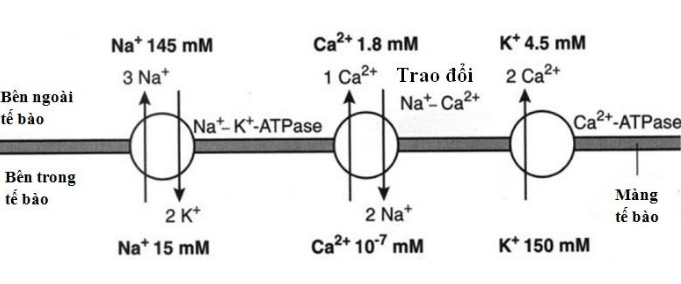
\includegraphics[scale=.4]{image/week1/h21.png}
    \end{center}
    \caption{Sự chênh lệch nồng độ của các ion Na, K, Ca trong cơ chế hình thành điện tâm đồ \cite{huongdanDTT}}
    \end{figure}
\end{center}\par
Tim người có 4 buồng để chứa và bơm máu. Hai phần nhỏ ở phía trên gọi là tâm nhĩ (vì trông giống lỗ tai). Hai phần dưới lớn hơn gọi là tâm thất. Máu theo tĩnh mạch từ cơ thể trở về tâm nhĩ phải, từ phổi trở về tâm nhĩ trái. Tâm nhĩ trái bóp bơm máu vào tâm thất trái, tâm nhĩ phải đưa máu vào tâm thất phải. Sau đó tâm thất phải bóp để bơm máu theo động mạch lên phổi và tâm thất trái bóp để bơm máu xuống cơ thể. Tim có khả năng hoạt động đều đặn và thứ tự như thế là nhờ một hệ thống các tế bào dẫn điện đặc biệt nằm trong cơ tim.\par
Trong tâm nhĩ bên phải có nút xoang nhĩ (sinoatrial node) gồm các tế bào có khả năng tự tạo xung điện (electric impulse). Xung điện này truyền ra các cơ chung quanh làm co bóp hai tâm nhĩ (tạo nên sóng P trên Điện Tâm đồ). Sau có dòng điện tiếp tục truyền theo 1 chuỗi tế bào đặc biệt tới nút nhĩ thất (atrioventricular node) nằm gần vách liên thất rồi theo chuỗi tế bào sợi Purkinje chạy dọc vách liên thất lan vào các cơ chung quanh (loạt sóng QRS) làm hai thất này co bóp. Sau đó xung điện giảm đi, tâm thất giãn ra (tạo nên sóng T).

\subsection{Các sóng cơ bản và sự hình thành phức bộ sóng}
Một chu kỳ tim biểu hiện trên điện tâm đồ là: sóng P, phức bộ QRS, sóng T, và sóng U (nếu có), hình dạng, thời gian kéo dài của sóng/phức bộ và cả thời gian giữa các thành phần với nhau đều có ý nghĩa đặc biệt quan trọng trong việc chẩn đoán.
\begin{center}
        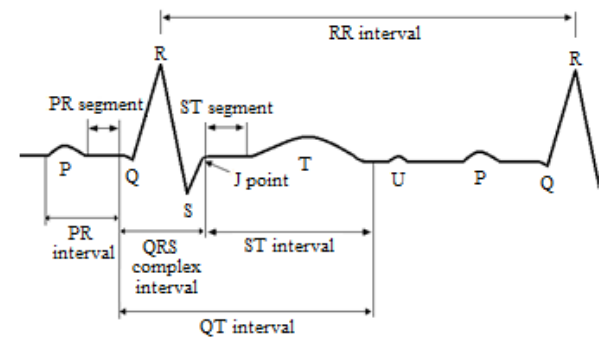
\includegraphics[scale=.4]{image/week1/h32.png}
        \begin{figure}[htp]
        \begin{center}
        \end{center}
        \caption{Tổng hợp những sóng cơ bản}
        \end{figure}
\end{center}

\subsubsection{Các sóng và phức bộ}
\textbf{Sóng P}\par
Sóng P hình thành do quá trình khử cực tâm nhĩ (cả nhĩ trái và nhĩ phải), bình thường biên độ của sóng P thường dưới 2mm (0.2mmV), và thời gian của sóng P là từ 0.08 đến 0.1 giây, việc tăng biên độ và kéo dài thời gian của sóng gợi ý đến một tình trạng tâm nhĩ lớn (tăng biên độ gợi ý lớn nhĩ phải. thời gian khử cực kéo dài gợi ý đến lớn nhĩ trái).\par
\textbf{Phức bộ QRS}\par
Phức bộ QRS thể hiện quá trình khử cực của tâm thất, tùy vào chiều khử cực và vị trí đặt điện cực mà trên giấy ghi sẽ cho thấy các phức bộ khác nhau, ưu thế sóng R hay S, bình thường QRS kéo dài từ 0.06 đến 0.1 giây.
\begin{itemize}
    \item Sóng Q là sóng âm đầu tiên của phức bộ QRS, sóng Q trên bệnh nhân bình thường thường nhỏ và ngắn (hình thành do quá trình khử cực vách liên thất), một sóng Q sâu (biên độ âm lớn) và kéo dài cho thấy một tình trạng hoại tử cơ tim (Trong nhồi máu cơ tim cũ hay nhồi máu cơ tim không có ST chênh lệch).
    \item Sóng R là sóng dương đầu tiên của phức bộ, và sóng âm sau nó là S, đây là hai sóng hình thành do khử cực thất, về bản chất là giống nhau, nếu điện cực đặt ở vị trị chiều khử cực hướng đến thì sóng R sẽ ưu thế, như trong chuyển đạo DII, V5, V6. Sóng R sẽ ưu thế hơn nếu chiều khử cực đi xa vị trí đặt điện cực như V1, V2.
\end{itemize}
\par
\textbf{Sóng T}\par
Là sóng theo sau phức bộ QRS, thể hiện quá trình tái cực muộn của 2 tâm thất, sóng T có giá trị rất lớn trong việc nhận định một tình trạng cơ tim thiếu máu.\par
\textbf{Sóng U}\par
Nguồn gốc sóng U vẫn chưa điện xác định rõ ràng, các giả thuyết đặt ra là:
\begin{itemize}
    \item Tái cực chậm sợi Purkinje.
    \item Tái cực kéo dài giữa cơ tim tế bào M (mid-myocardial cell).
    \item Sau kết quả điện thế của trương lực cơ trong các thành tâm thất.
\end{itemize}
Bình thường không thấy sóng U trên điện tâm đồ, nếu có thì là sóng nhỏ sau sóng T, sóng U đảo ngược hay nhô cao nhọn gặp trong rất nhiều loại bệnh lý tim (bệnh mạch vành, tăng huyết áp, bệnh van tim, tim bẩm sinh, bệnh lý cơ tim, cường giáp, ngộ độc, rối loạn điện giải,...)
\subsubsection{Các đoạn - khoảng}
\textbf{Khoảng PQ}\par
Là thời gian dẫn truyền từ nhĩ đến thất, bình thường từ 0.12 - 0.2 giây, việc kéo dài thể hiện quá trình chậm dẫn truyền (do bị block), PQ ngắn sẽ gợi ý đến một hội chứng kích thích sớm (Wolf-Parkinson-White)\par
\textbf{Đoạn ST}\par
Ý nghĩa là giai đoạn tái cực thất sớm, thời gian của ST thường không quan trọng bằng hình dạng của nó, bình thường ST nằm chênh lệch lên hoặc chênh xuống khỏi đường đẳng điện rất ít. đoạn ST cực kỳ quan trọng trong việc chẩn đoán nhồi máu cơ tim.\par
ST gọi là chênh lệch nếu cao hơn đường đẳng điện 1mm ở chuyển đạo chi và hơn 2mm ở chuyển đạo trước ngực\par
ST gọi là chênh xuống khi nằm dưới đường đẳng điện hơn 0.5mm\par
\textbf{Đoạn QT}\par
Là thời gian tâm thu điện học của tâm thất, khoảng giá trị bình thường của QT phục thuộc vào tần số tim, QT kéo dài bất thường có liên quan với tăng nguy cơ loạn nhịp thất, đặc biệt là xoắn đỉnh. Gần đây, hội chứng QT ngắn bẩm sinh đã được tìm thấy có liên quan với tăng nguy cơ rung nhĩ và thất kịch phát và đột tử do tim.

\subsection{Các chuyển đạo thông dụng}

\subsubsection{Điện trường tim}
Cơ thể con người là một môi trường dẫn điện; vì thế, dòng điện do tim phát ra được dẫn truyền khắp cơ thể, ra tới da, biến cơ thể thành một điện trường của tim. Nếu ta đặt hai điện cực lên bất cứ hai điểm nào đó có điện thế khác nhau của điện trường đó, ta sẽ thu được một dòng điện thể hiện hiệu thế giữa hai điểm đó và gọi là một chuyển đạo hay đạo trình (lead). Nó hiện ra trên máy ghi bằng một đường cong điện tâm đồ có một hình dạng nào đó tùy theo địa điểm đặt các điện cực. Đường thẳng nối hai địa điểm đặt điện cực trên cơ thể gọi là trục chuyển đạo.

\subsubsection{Chuyển đạo mẩu:}
\begin{center}
    \begin{figure}[htp]
    \begin{center}
    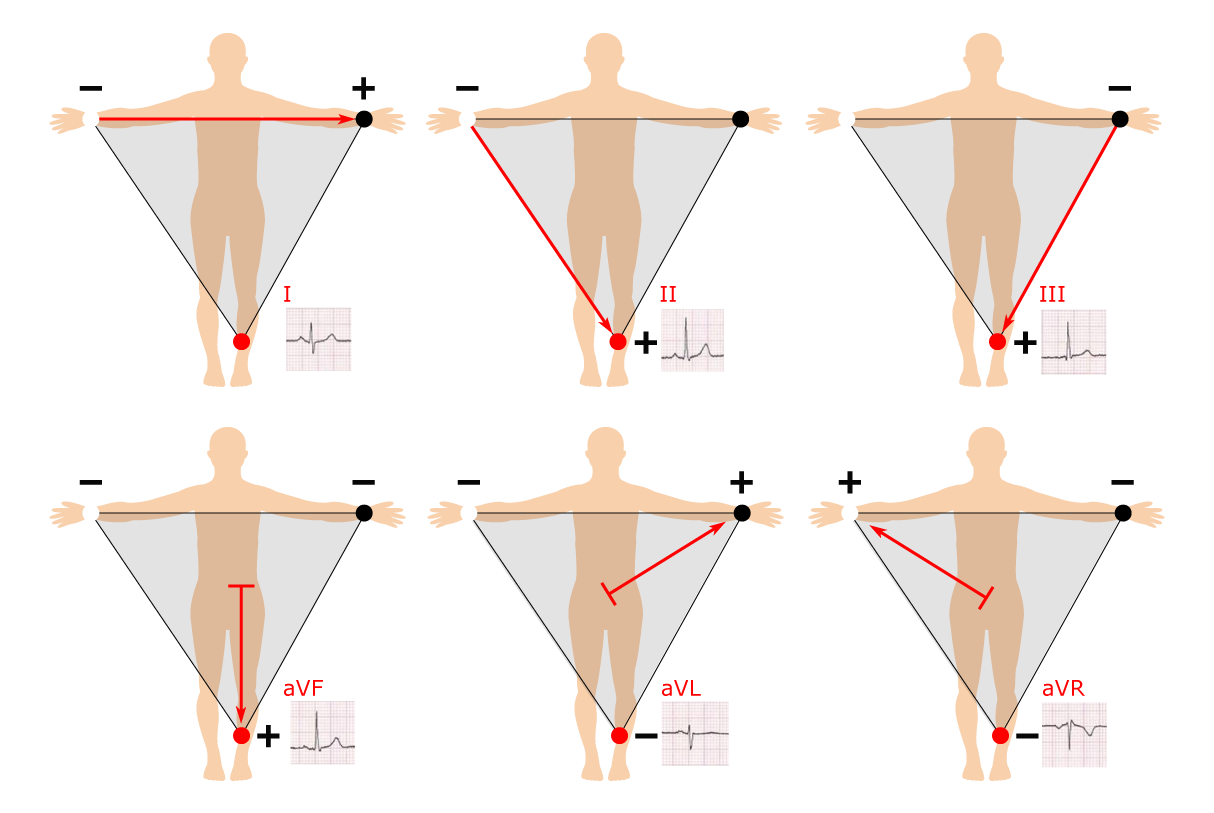
\includegraphics[scale=.2]{image/week1/chuyendaochi.png}
    \end{center}
    \caption{Chuyển đạo chi \cite{chuyendao}}
    \end{figure}
\end{center}
Tất cả 6 chuyển đạo: D1, D2, D3, aVR, aVL, aVF được gọi chung là các chuyển đạo ngoại biên vì đều có điện cực thăm dò đặt ở các chi. Chúng hỗ trợ cho nhau “dò xét” các rối loạn của dòng điện tim thể hiện ở bốn phía xung quanh quả tim trên mặt phẳng chắn (frontal plane).
\begin{center}
    \begin{figure}[htp]
    \begin{center}
    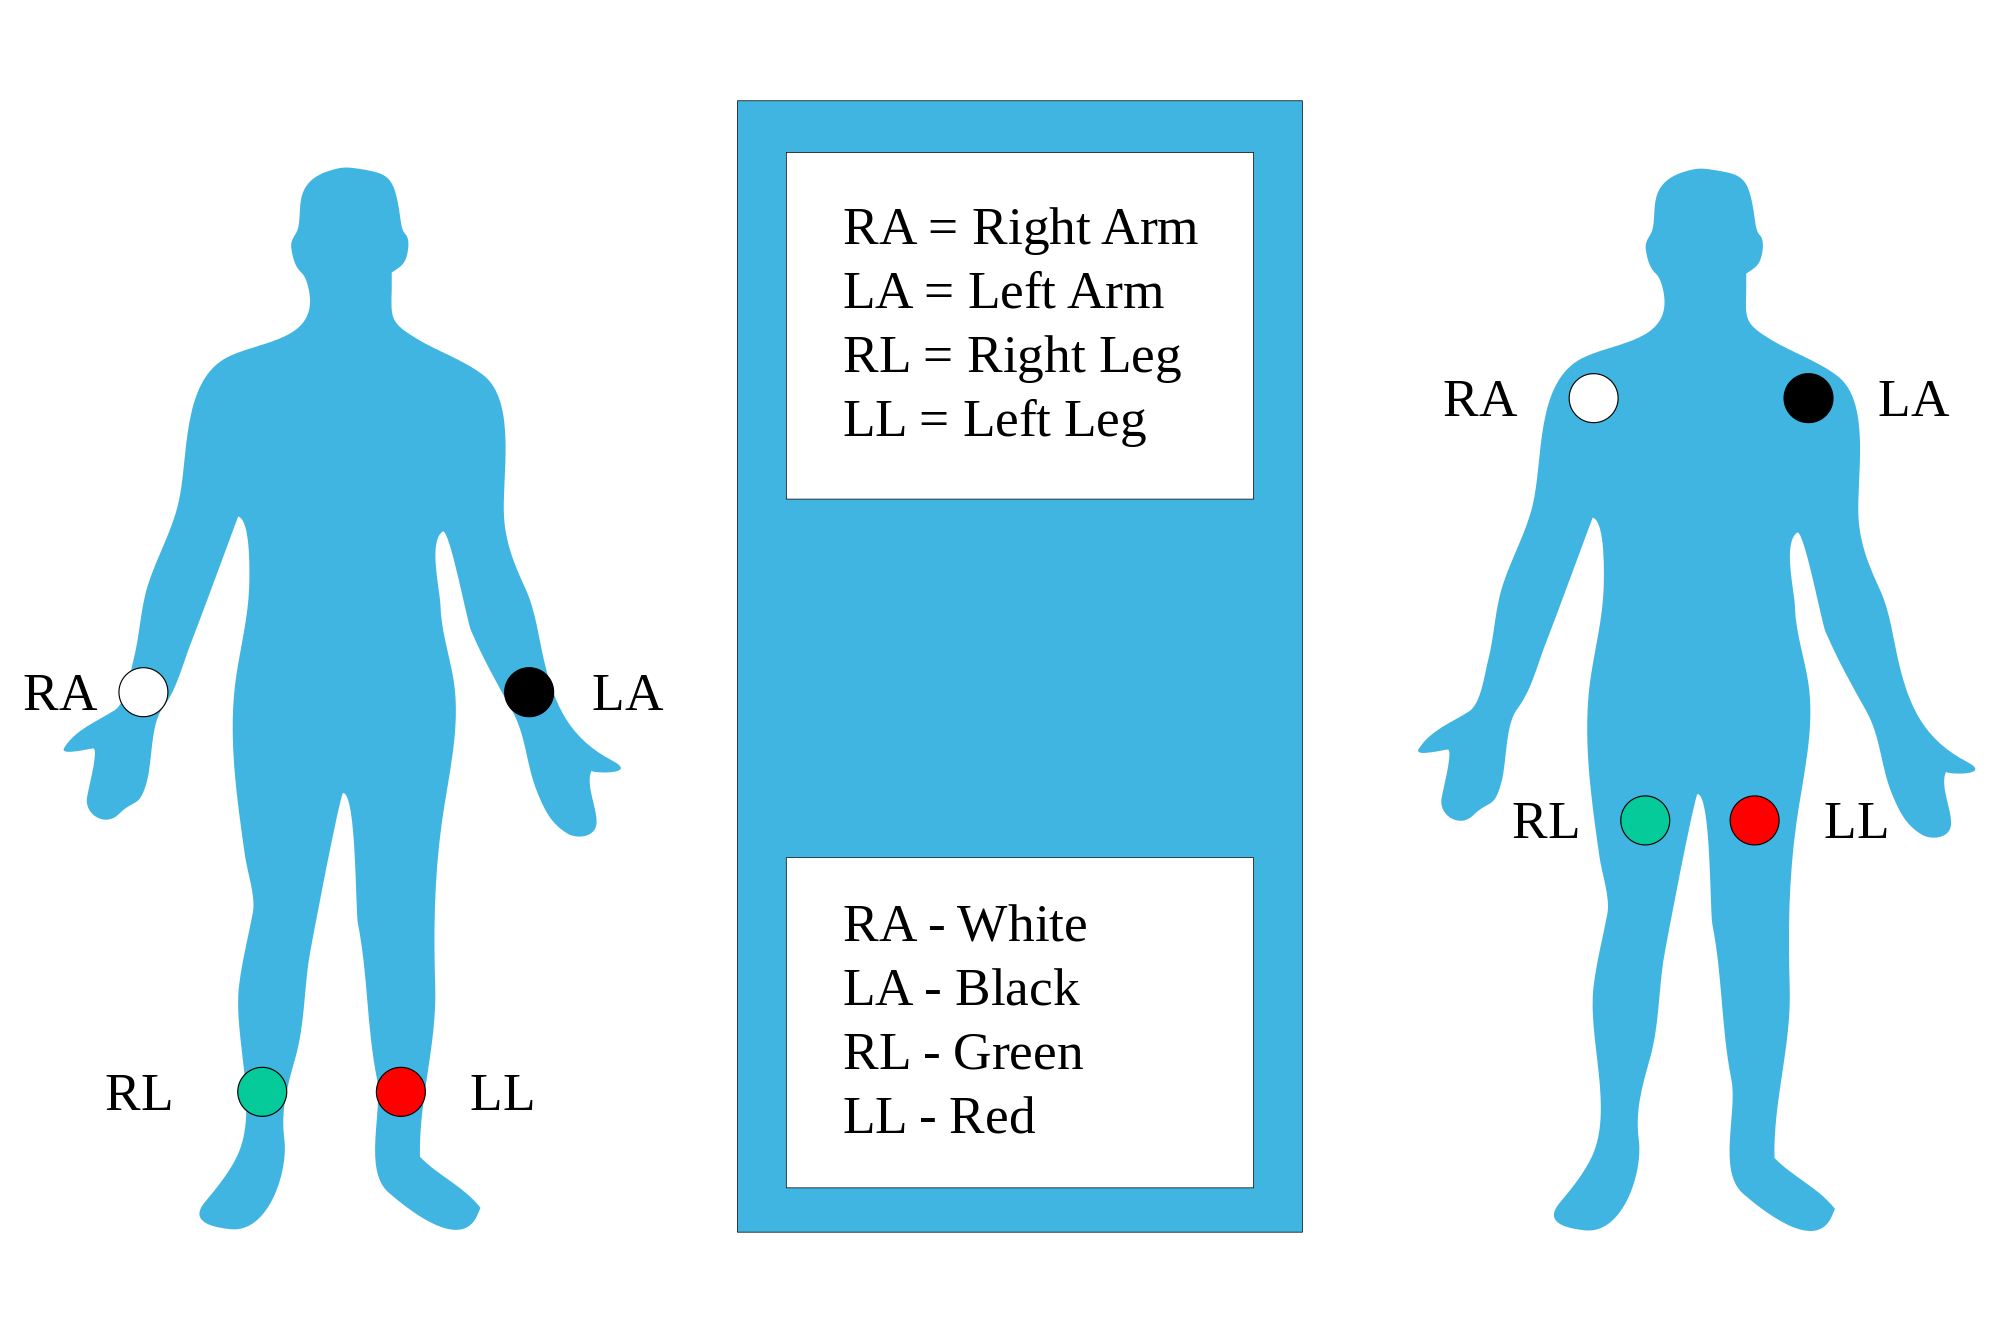
\includegraphics[scale=.12]{image/chapter1/2000px-Limb_leads.png}
    \end{center}
    \caption{Các vị trí đặt điện cực để đo ECG}
    \end{figure}
\end{center}

\subsubsection{Chuyển đạo trước tim:}
\begin{center}
    \begin{figure}[htp]
    \begin{center}
    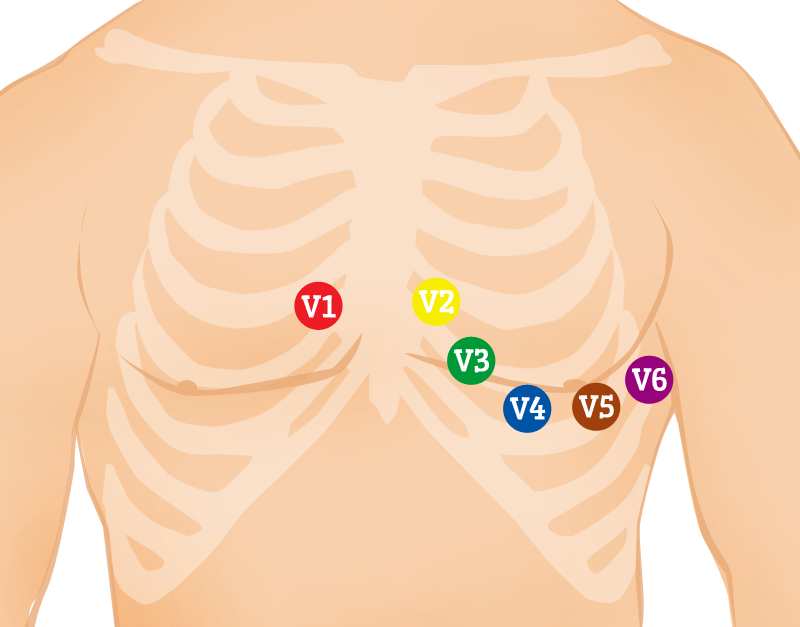
\includegraphics[scale=.25]{image/week1/chuyendaotruocnguc.png}
    \end{center}
    \caption{Chuyển đạo trước tim }
    \end{figure}
\end{center}
Người ta thường ghi đồng loạt cho bệnh nhân 6 chuyển đạo trước tim thông dụng nhất, kí hiệu bằng chữ V (voltage) kèm theo các chỉ số từ 1 đến 6.(V1, V2,…,V6).

\subsubsection{Một số chuyển đạo khác:}
V7, V8, V9(điện cực ở mé trái và sau lồng ngực dùng để thăm dò thất trái), V3R, V4R, V5R, V6R(điện cực ở mé phải lồng ngực dùng để nghiên cứu thất phải hay tim sang phải), chuyển đạo thực quản (Kí hiệu VOE), chuyển đạo trong buồng tim, điện đồ His.

\subsection{Đo điện tâm đồ}
\subsubsection{Đo điện tâm đồ truyền thống}
Định dạng chuẩn của một điện tâm đồ là điện tâm đồ được ghi lại trên một khổ giấy
.Để đánh giá thời gian dài hay ngắn và biên độ cao hay thấp của các làn sóng điện tâm đồ, người ta đinh chuẩn: 
\begin{itemize}
    \item Vận tốc 25mm/s thì mỗi ô 1mm có giá trị 0,04s.
    \item Theo chiều ngang 1 ô lớn tương ứng với 1000ms.
    \item Theo chiều dọc 1 ô lớn tương ứng 500mV.
\end{itemize}
\begin{center}
    \begin{figure}[htp]
    \begin{center}
    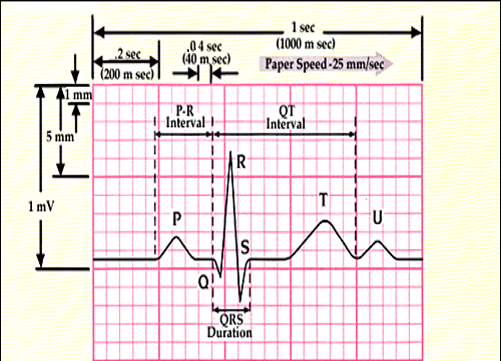
\includegraphics[scale=.6]{image/week1/new_ecg_paper.png}
    \end{center}
    \caption{Hình ảnh một chu kỳ sóng được đo theo kích thước khổ giấy, bác sĩ căn cứ vào ô trên giấy để phát hiện bất thường ở ECG \cite{ecggiay}}
    \end{figure}
\end{center}
\subsubsection{Đo điện tâm đồ bằng thiết bị di động thông minh (Apple Watch Series 4)}
Tính năng ECG hay còn gọi là đo điện tâm đồ đã chính thức có thể sử dụng trên Apple Watch Series 4 để phát hiện nhịp tim bất thường và chẩn đoán các bệnh tim nghiêm trọng.
\begin{center}
    \begin{figure}[htp]
    \begin{center}
    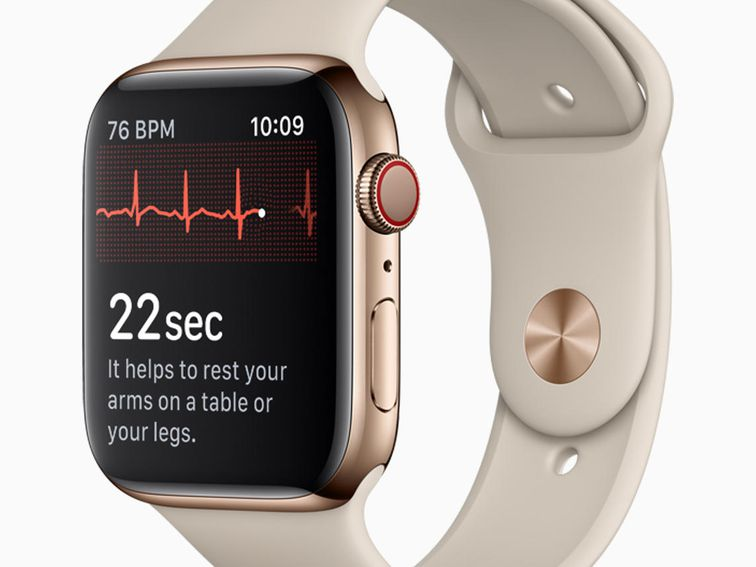
\includegraphics[scale=.3]{image/chapter1/apple-watch-series4-ecg-crown-09122018.jpg}
    \end{center}
    \caption{Apple Watch Series 4}
    \end{figure}
\end{center}
% \section{Đọc một điện tâm đồ}
% \subsection{Những bước phân tích trước khi đọc một điện tâm đồ}
% Điện tâm đồ (ECG) là một đường cong ghi lại các biến thiên của các điện lực do tim phát ra trong khi hoạt động co bóp.\cite{huongdanDTT}

% \begin{enumerate}
%     \item Trước khi đọc điện tâm đồ, phải nắm vững tuổi, giới tính, chẩn đoán lâm sàng của bệnh
%     nhân. Ngoài ra, còn nên biết thêm sơ lược bệnh án, hình ảnh X quang, các kết quả xét nghiệm khác và nhất là hai vấn đề sau đây:
%     \begin{itemize}
%         \item Khổ người bệnh nhân gầy béo, cao thấp ảnh hưởng rất nhiều đến tư thế tìm và biên độ sóng, nó ảnh hưởng nhiều đến chẩn đoán dày thất.
%         \item Có đang dùng thuốc trợ tim hay thuốc chống loạn nhịp dài ngày không? Nhất là digitan và quinidin… vì các thuốc này tác động rất nhiều đến hình dạng điện tâm đồ và dễ làm sai lạc chẩn đoán cơ bản.
%     \end{itemize}
%     \item Kiểm tra kỹ thuật ghi điện tâm đồ, phát hiện ghi sai, ảnh hưởng tạp, milivôn lấy đúng 1cm
%     hay không? Tốc độ ghi bao nhiêu? Nghĩa là các đường kẻ dọc cách nhau bao nhiêu phần trăm
%     giây
%     \item Nhịp tim: bước vào đọc điện tâm đồ trước hết bao giờ cũng phải xem nhịp xoang hay
%     không xoang? Có những rối loạn nhịp tim gì? Đừng bao giờ quên tính tần số tim. Nếu có blốc
%     nhĩ-thất thì phải tính riêng cả tần số nhĩ.
%     \item Trục điện tim với góc alpha, tư thế tim.
%     \item Hình dạng các sóng: đọc đồng thời ở cả 12 chuyển đạo thông dụng:
%     \begin{itemize}
%         \item Sóng P: chiều cao (biên độ), chiều rộng (thời gian), hình dạng (âm, dương, hai pha, móc).
%         \item Khoảng PQ dài bao nhiêu?
%         \item Phức bộ QRS: biên độ và thời gian chung và riêng của sóng Q, hình dạng (móc…).
%         \item Riêng với V1 và V5 thì tìm thêm thời gian xuất hiện nhánh nội điện.
%         \item Đoạn ST có chênh không?
%         \item Sóng T (và sóng U): dạng (dương, âm hay hai pha), biên độ.
%         \item Khoảng QT dài bao nhiêu?
%     \end{itemize}
%     \item Kết luận chẩn đoán: về tổn thương cơ tim và về rối loạn nhịp tim.
% \end{enumerate}
